\documentclass{elsarticle}
%%\documentclass[review]{elsarticle}

\usepackage{float}
\usepackage{lineno,hyperref}
\usepackage{graphicx}
\usepackage{listings}
\usepackage{subfigure} 
\modulolinenumbers[5]

\bibliographystyle{elsarticle-num}

\begin{document}

\begin{frontmatter}

\title{A Case Study of the Component and Connector Modeling Language EmbeddedMontiArc}
\tnotetext[mytitlenote]{}

%% Group authors per affiliation:
\author{Haller, Heithoff}
\address{Supervised by: Michael von Wenckstern and Bernhard Rumpe \\ Software Engineering, RWTH Aachen University}



\begin{abstract}
(Abstract by Philipp Haller)
The magnitude and quantity of software projects rises constantly, as software development needs spread among scientific and technical disciplines. Domain Specific Languages (DSLs) show to provide solutions for specialized contexts. EmbeddedMontiArc is a DSL for cyber physical systems.
This paper represents a case-study, evaluating the ease of use and re-usability of EmbeddedMontiArc for reactive systems by presenting models for the games Pacman and Supermario. Games are highly reactive systems were entities controlled by the player react to a changing environment and try to reach goals, thus can provide a good testing ground for actual systems.
From the models presented it is concluded that EmbeddedMontiArc is suitable for cyber-physical systems, but still not flawless.


\end{abstract}

\begin{keyword}
EmbeddedMontiArc, Component \& Connector Models, Case Study, Supermario, Pacman
\end{keyword}

\end{frontmatter}

\linenumbers


\newpage
\section{Introduction (by Philipp Haller)}
\label{sec:intro}
The magnitude and quantity of software projects rises constantly, as software development needs spread among scientific and technical disciplines. Since not all languages are suitable for all occasions and others may provide too much features to be efficient for a specific purpose, Domain Specific Languages (DSLs) are developed. DSLs are languages tailored specifically to a certain objective.
EmbeddedMontiArc, a specific DSL for cyber-physical systems is evaluated in this paper. It will be introduced in more detail in section \ref{sec:context} together with the used tools. This section forms a general introduction and will present the research questions.
Thereafter the approach will be presented in section \ref{sec:approach}. Section \ref{sec:implementation} depicts the simulator integration and the developed models. In section \ref{sec:evaluation} the evaluation is presented, concluded by a conclusion in section \ref{sec:conclusion}.

In general most problems can be sorted into two categories. The first being data based problems, where huge amounts of data are processed and no hard real time capabilities are necessary. An example for such a problem is Google's or Amazon's search system. The other problem category consists of reactive systems which operate on very little data and must return output with hard time constraints. In this paper EmbeddedMontiArc is evaluated towards its capabilities for the second category. The language is well tested on the autopilot project of a self driving car (see \cite{emademo}), but has few other running examples.
The following research questions were formulated to specify evaluation topics:

\begin{itemize}
	\item RQ1: Is EmbeddedMontiArc suitable reactive systems in domains other than the automotive industry?
	\item RQ2: Is it possible to integrate other simulators in a recent amount of work?
	\item RQ3: What kind of background knowledge is needed to model C\&C in EmbeddedMontiArc?
	\item RQ4: What features are good and what are not suited?
\end{itemize}

To answer these research questions two groups are formed who develop different models in EmbeddedMontiArc and share their experience while doing so. To ensure a similar experience to real reactive cyber physical systems, two games were selected.
Games were selected, because most games are real-time problems with a changing environment and limited inputs, while requiring immediate responses.
The games chosen for this paper are Pacman and Supermario.  Both games are 2D arcade games where a figure is controlled by a player in a setting where some types of enemy entities exist. In the case of Pacman the level is completely visible and enemies consist of ghosts roaming the level. The level is failed once the ghosts touch the player. Goal of the game is to collect or "eat" all dots in the level.
Supermario is a side-scrolling platform game were the level is revealed as the player progresses. Main goal of Supermario is to bring the player figure all the way through to the end of the level, while either evading or defeating the different enemy types. The players progress is rated via a scoring system, where enemy defeats and collectibles are assessed.
Goal for both models developed in this paper is to solve a level in their respective game.

The finished models can be observed playing Pacman and Supermario autonomouosly on the websites \\
\url{https://embeddedmotiarc.github.io/SuperMario/Pacman/}\cite{pacmanmodel} \\
and \\
\url{https://embeddedmontiarc.github.io/SuperMario/supermario/simulation.html}\cite{mariomodel}.


\section{Context (by Philipp Haller)}
\label{sec:context}
The following section consists of three parts. The first one is a brief introduction to C\&C models. The tools used for this study follow up second. Lastly, the used case study method is presented.

\subsection{C \& C models}

In the following a short introduction in Connector and Component (C\&C) model based software development is given. C\&C modeling divides a task into Components and Connectors.

A \emph{Component} represents a computation. It has predefined inputs and outputs, where the output data is obtained by some kind of mathematical transformation of the input data. A \emph{Connector} represents interaction mechanisms by connecting outputs with inputs. By making this division, the paradigm ensures modularity and therefore re-usability.
It can be used for modeling software with high demands for testing and verification such as software for self-driving vehicles \cite{WencksternCCViP}\cite{WencksternSimFrame}.
Another benefit is that a graphical representation is always possible and more efficiently obtainable compared to other text based development, especially non model driven development. The structure of C\&C models also benefits code generation techniques in order to transform models into source code for various target systems.
Well established examples of C\&C modeling and development are SysML\cite{sysml}, AADL\cite{aadl}, Simulink\cite{simulink} and Labview\cite{labview}. The latter two are used in the automotive domain to model behaviour of Electronic Control Units (ECUs) and test their functionality.

\subsection{MontiCore and EmbeddedMontiArc}

MontiCore \cite{HR17}, MontiCAR \cite{KRRW17} and EmbeddedMontiArc \cite{HKK+18} are tools developed by the Chair of Software Engineering of RWTH Aachen University\cite{serwth}.
\emph{MontiCore} is a language workbench intended for agile and model-driven software development. Its primary objective is to enable efficient development of Domain Specific Languages (DSLs) which enhance the development process for Domain Experts. 
\emph{MontiCAR} is a composition of such DSLs, used as an language set for Cyber-Physical Systems \cite{seminarArmin}. Figure \ref{fig:MontiCAR} shows the DSLs which are part of MontiCar and their respective connections.
\begin{figure}
	\centering
	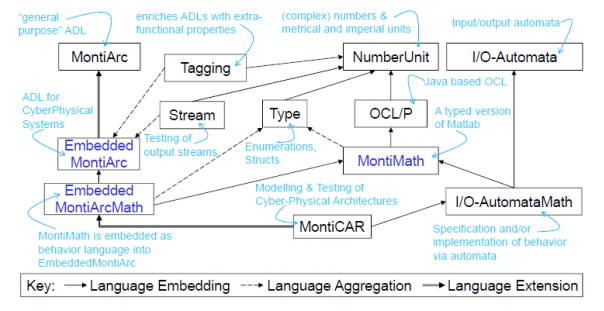
\includegraphics[width=\textwidth]{pictures/MontiCarOverview.PNG}
	\caption{Composition of MontiCAR language family\cite{seminarArmin}}
	\label{fig:MontiCAR}
\end{figure}
The components directly used in this studies implementation are EmbeddedMontiArc, EmbeddedMontiArcMath and Stream.
\emph{EmbeddedMontiArc} represents the core language of MontiCar. It implements a C\&C DSL which can be used to write C\&C models, verify, test and deploy them to another architecture. Due to its modularity different simulators and Stream tests can be integrated. See the chapter modeling for more information. Figure \ref{fig:EMontiArc} depicts a usage of the EmbeddedMontiArc DSL.

\begin{figure}[!h]
	\centering
	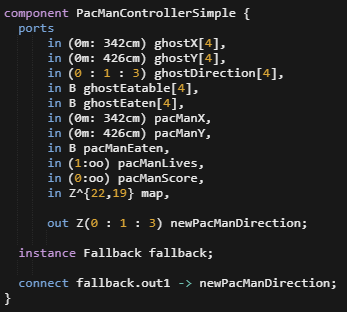
\includegraphics[scale=0.70]{pictures/EMA.PNG}
	\caption{Example Component with Connectors}
	\label{fig:EMontiArc}
\end{figure}

\emph{EmbeddedMontiArcMath} is a DSL for implementing mathematical expressions, thus used for transforming the input values of a Component into its output values. It is also able to declare other variables than the defined inputs and logical structures like if-statements and loops. Example usage of EmbeddedMontiArcMath is shown in figure \ref{fig:EMontiArcMath}.

\begin{figure}[!h]
	\centering
	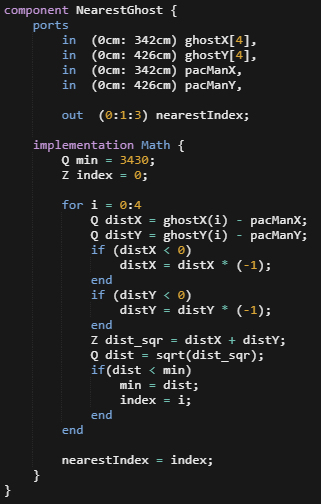
\includegraphics[scale=0.7]{pictures/EMAMath.PNG}
	\caption{Example EmbeddedMontiArcMath implementation}
	\label{fig:EMontiArcMath}
\end{figure}

The \emph{Stream} DSL allows to implement test cases by defining the expected output values for a given input. Multiple values can be tested in one Stream test, as shown in figure \ref{fig:EMAStream} which shows an example stream test for a sum function. Thy syntax of this DSL holds the following items: 
\begin{itemize}
	\item The package which also holds the component (de.rwth...)
	\item The test's name (Sum)
	\item The name of the component to test (Sum)
	\item Values for each input port (t1 and t2)
	\item A line with the values for at least one output port (result)
\end{itemize}
The values for one port are separated by ticks. Each tick stands for one execution cycle. This way a component can be tested over several cycles which gets important if the component's behavior is dependent on previous execution cycles. In addition the \textit{+/-} allows inaccuracy in the results.

\begin{figure}[!h]
	\centering
	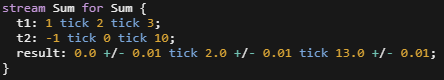
\includegraphics[scale=0.75]{pictures/EMAStream.PNG}
	\caption{Example Stream implementation]}
	\label{fig:EMAStream}
\end{figure}



\subsection{Performing a Case Study in Software Engineering}
This study roughly follows the guidelines stated by Runeson and Hoest \cite{CaseStudyGuidelines} by presenting the objective, the specific case, method and acquiring both quantitative and qualitative data. Quantitative data is acquired by asking a set of predefined questioned and answering them on a scale from 1 to 10. The qualitative data is obtained via requiring subjects to formalize how they gave the quantitative rating.
The quantitative data is analyzed by calculating the mean of each question, and the quantitative by summarizing the subject's writings.



\section{Approach}
\label{sec:approach}
To address \textbf{RQ1} and \textbf{RQ3} two groups were assigned the task to model a controller for Pacman and Supermario respectively and interview the results afterwards. The first group (Pacman) consists of a subject who is familiar with EmbeddedMontiArc and the second group (Supermario) consists a subjects who have no experience with EmbeddedMontiArc. These groups were selected random among the students of a computer science seminar.
\subsection{Stream Testing (by Heithoff)}

EmbeddedMontiArc comes along with stream tests in order to check a component against a condition as stated in the previous chapter.
We can use those tests to define the conditions the controllers need to fulfill. Those conditions are taken from use cases scenarios. For Pacman the most general acceptance test would be to never let the Pacman die. Due to the fact that stream tests cannot be defined unlimited and that this test might be hard to fulfill the following deterministic tests for Pacman and Supermario were defined.

\subsubsection{Pacman (by Heithoff)}
The tests are taken from use case scenarios as stated before. In this section the process of deriving the stream test from a scenario is presented once and then a few conditions are framed. \newline

\emph{Deriving a Stream Test} \newline
In fig. \ref{fig:PacmanFleeing} a scenario is shown where the only option for Pacman is to flee to the left in order to not collide with the pink and blue ghost. The values of the ghosts and Pacman are partially listed in listing \ref{lst:pmStreamValues}. Together with the remaining values this concludes to the stream test shown below \ref{lst:pmStreamTest}.
\newline 
\begin{figure}[!h]
	\centering
	\subfigure[]{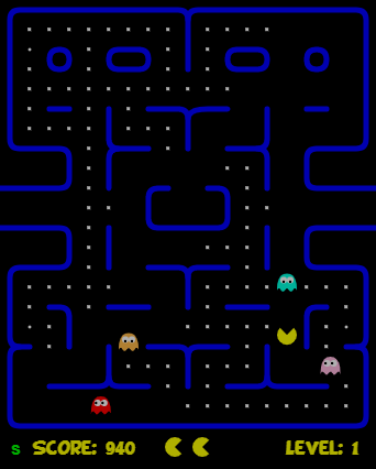
\includegraphics[width=0.49\textwidth]{pictures/Pacman/StreamTests/2/Bild1.PNG}} 
	\subfigure[] {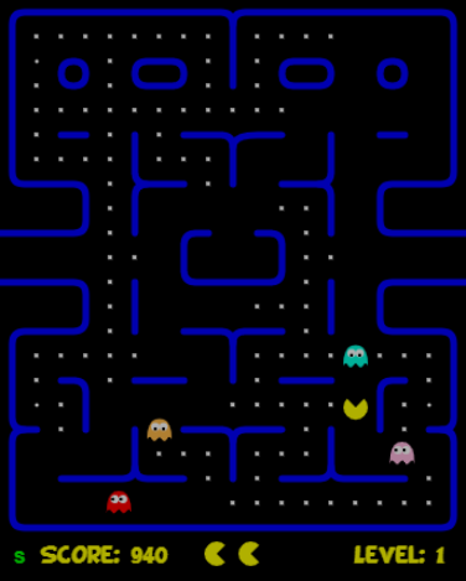
\includegraphics[width=0.49\textwidth]{pictures/Pacman/StreamTests/2/Bild2.PNG}} 
	\subfigure[]{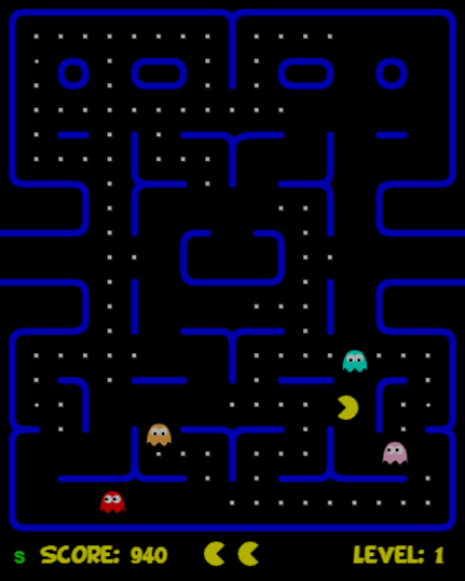
\includegraphics[width=0.49\textwidth]{pictures/Pacman/StreamTests/2/Bild3.PNG}} 
	\subfigure[]{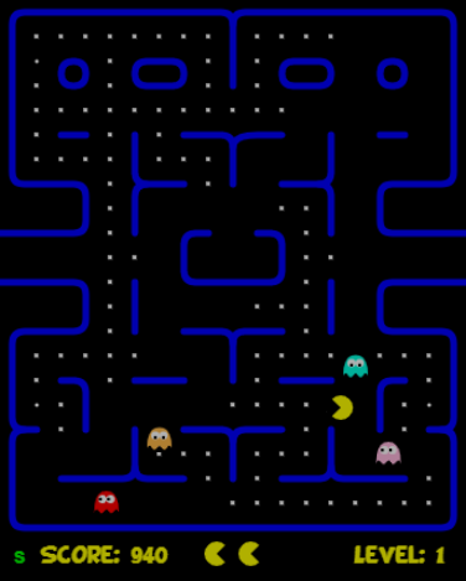
\includegraphics[width=0.49\textwidth]{pictures/Pacman/StreamTests/2/Bild4.PNG}} 
	\caption{Pacman has to move left to avoid colliding with the ghosts} 
	\label{fig:PacmanFleeing}
\end{figure}

\begin{lstlisting}[caption={Values for the stream test},label=lst:pmStreamValues]
(a)
  Pacman: (15m, 17.2m) 
  Pink Ghost: (17m, 19m) 
  BlueGhost: (15m, 14.8m) 
  newDir: 0
(b)	
  Pacman: (15m, 17m) 
  Pink Ghost: (16.8m, 19m) 
  BlueGhost: (15m, 15m) 
  newDir: 0
(c)	
  Pacman: (14.8m, 17m) 
  Pink Ghost: (16.6m, 19m) 
  BlueGhost: (15m, 15.2m) 
  newDir: 2
(d)	
  Pacman: (14.6m, 17m) 
  Pink Ghost: (16.4m, 19m)
  BlueGhost: (15m, 15.4m)
  newDir: 2
\end{lstlisting}

\begin{lstlisting}[caption={Stream test for the scenario above},label=lst:pmStreamTest]
package de.rwth.Pacman;
stream Test1 for PacmanWrapper {
  ghostX: [5.4m,15m,17m,7m] tick [5.2m,15m, ...
  ghostY: [21m,14.8m,19m,17.2m] tick [21m,15m, ...
  ghostDirection: [2,1,2,1] tick [2,1,2,1] tick ...
  ghostEtable: [false, false, false, false] tick ...
  ghostEaten: [false, false, false, false] tick ...
  PacmanX: 15m tick 15m tick 14.8m tick 14.6m;
  PacmanY: 17.2m tick 17m tick 17m tick 17m;
  PacmanEaten: false tick false tick false tick false;
  PacmanLives: 3 tick 3 tick 3 tick 3;
  PacmanScore: 0 tick 0 tick 0 tick 0;
  map: [0,0,0,0,0,0,0,0,0,0,0,0,0,0,0,0,0,0,0; ...
  newPacmanDirection: 0 tick 0 tick 2 tick 2;
}
\end{lstlisting}
\emph{Some other tests}\newline
To formulate just some tests, here are a few examples:
\begin{itemize}
	\item If Pacman is located at an intersection and ghosts are coming from two sides, Pacman should walk to a safe path.
	\item If Pacman is located at an intersection and ghosts are at the top path and are all eatable, Pacman should walk this path.
	\item If Pacman is located at an intersection and there are ghosts from 3 directions and in the other direction there is a ghost facing away from Pacman, Pacman should walk this direction.
	\item If there are no ghosts nearby, Pacman should walk the direction with the largest biscuit/coin value.
\end{itemize}

Those scenarios can be tested easily within a few ticks via stream testing.

\subsubsection{Supermario (by Philipp Haller)}
\input{approach-Supermario}

\subsection{Preparations (by Haller and Heithoff)}
The code of the Pacman emulator \cite{PacmanLink} and Supermario emulator \cite{marioLink} is available in HTML5 and JavaScript. C\&C-Components in EmbeddedMontiArc can be translated to C++ code and then to a web assembly \cite{KRSvW18} which uses JavaScript. This JavaScript file can be given inputs according to the component and calculates the outputs on execution. To combine these two files, there is an additional interface needed to extract the information for the inputs out of the emulator and then give the calculated outputs into the emulator.
For the purpose of implementing the controllers the subjects were assigned to use the EmbeddedMontiArcStudio.
EmbeddedMontiArcStudioV1.6.2 did neither support a simulator for Pacman nor a simulator for Supermario. So an additional step to answer RQ2 \textit{Is it possible to integrate other simulators in a recent amount of work} it for the groups to integrate the simulators into the EmbeddedMontiArcStudio.

In order to be able to do so, group Pacman is instructed by an expert (Jean-Marc) which files need modification and what to add. After that this group instructed the second group the same way.




\section{Case Study Execution}
\label{sec:implementation}

In this chapter the implementation is described. First, the necessary steps for integrating a new Simulator into the IDE are shown. In the second part the modeling of the controllers for Pacman and Supermario are discussed.


\subsection{Integration of Simulator into IDE (Introduction by Philipp Haller)}

As the participants of the use-case study were divided into two groups, the first group dealt with the IDE integration of the Pacman simulator after being instructed by an EMA professional.
After successful integration this first group wrote a step-by-step instruction list. The second group used this list to integrate the Supermario simulator into the IDE. Details are given in the following.

\subsubsection{Integration at the example of Pacman (by Malte Heithoff)}
\begin{figure}
	\caption{Main options for the Pacman project in the ide}
	\label{fig:idePacmanTop}
	\centering
	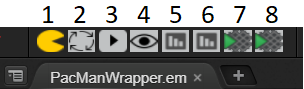
\includegraphics[scale=0.55]{pictures/IDE/IDETop.png}
\end{figure}
To integrate a simulator into the EmbeddedMontiArcStudio several steps were necessary. In figure \ref{fig:idePacmanTop} you can see the top view of the EmbeddedMontiArc's IDE. The five added features here are as follows:
\begin{itemize}
	\item[1.] Open a new tab where you can play a normal game of Pacman
	\item[2.] Generate the WebAssembly of the main component
	\item[3.] Open a new tab in which the simulation of the component takes place
	\item[4.] Generates the visualization of the main component and shows it in a new tab
	\item[5.] Generates the reporting of all components and shows it in a new tab
	\item[6.] Generates the reporting of all components with stream test results and shows it in a new tab
	\item[7.] Run all tests in the repository and show their results
	\item[8.] Run a single test and show its result
\end{itemize}
The features needed to be implemented properly in different places in order to work along the logic of the ide. Each one calls a batch script which again runs the jar for the demanded task for the specific files. In addition, for feature 1 and 2 extra plugins were required which got implemented by the expert group Pacman and could be reused for Supermario.



\subsection{Modeling}

This chapter introduces the models of Pacman and Supermario respectively.
The models should always follow certain rules defined in the EmbeddedMontiArc documentation (see \cite{emadoc}). The math implementation of all atomic components should be short and have a short runtime. This way not only the clarity of the code is enhanced but also the runtime of the components is fixed. C\&C models should, at some point, be runnable on microchips and due to the fact that those models are designed for real-time systems the runtime has to be fix.
To achieve this a lot of functionality can be extracted into subcomponents. In general, loops should be avoided and split up into subcomponents if possible. Because while loops are not ensured to terminate, those should never be used.

\subsection{Pacman (by Heithoff)}
In the following the model for the Pacman controller is presented. The goal is to collect as many biscuits and coins as possible and to avoid the ghosts. After introducing the interface which is used here two controllers for Pacman are shown. There is a simple controller which was used in the early stages of the IDE integration to test everything and then a more complex controller that can actually survive a few levels.

\subsubsection{Interface}
\begin{figure}
	\caption{Visualization of the Pacman wrapper}
	\label{fig:visPacmanWrapper}
	\centering
	\includegraphics[scale=0.7]{pictures/VisualizationPacmanWrapper.png}
\end{figure}
\begin{lstlisting}[label=lst:pacmanWrapper, caption=Interface of the Pacman Wrapper, morekeywords={ports, port, connect, in, out, instance, ->},
frame=single]
ports 
	in Z(0cm: 180cm) ghostX[4],
	in Z(0cm: 210cm) ghostY[4],
	in Z(0 : 1 : 3) ghostDirection[4],
	in B ghostEatable[4],
	in B ghostEaten[4],
	in Z(0cm: 180cm) pacManX,
	in Z(0cm: 210cm) pacManY,
	in B pacManEaten,
	in Z(0:oo) pacManLives,
	in Z(0:oo) pacManScore,
	in Z^{22,19} map,
	out Z(0 : 1 : 3) newPacmanDirection;
\end{lstlisting}
The project's main component is PacmanWrapper. The main task of the wrapper is to provide a shared interface. Listing \ref{lst:pacmanWrapper} shows the input and output ports. As for the inputs, the ghosts' and the Pacman's position are given, the direction the ghosts are facing, information about the ghosts' vulnerability, as well as the current map. The only output port is the new direction the Pacman should walk. \newline
The wrapper also holds the current controller. This way the controller is easily exchangeable without changing any of the code needed for the ide. All input ports of the wrapper are connected to the corresponding ports of the controller and the output port of the controller is also connected to the output port of the wrapper. \newline
To connect the web assembly of the main component with the Pacman emulator a new JavaScript file was created. Its main functionalities is to extract the needed informations out of the emulator, pass it to the web assembly, execute it and then give the output back to the emulator. In order to be able to extract needed information out of the emulator some modifications were needed. In its original state the emulator did not offer access to the current game object, thus the PACMAN class was extended by these functions. Due to the fact Pacman is a playable game, its input is given as a key-press-event in JavaScript. So the output of the web assembly, which is a number from 0 to 3, is mapped to a corresponding key-press-event which then gets triggered. The emulator is running with 30 frames per second, which also leads to 30 iterations of the game per second. Because the emulator is running asynchronously the component is executed at a double of that rate in order to track every position change.

\subsubsection{C\&C modeling - Pacman (simple)}
\begin{figure}
	\caption{Visualization of the Pacman controller (simple)}
	\label{fig:visPacmanSimple}
	\centering
	\includegraphics[scale=0.7]{pictures/VisualizationPacmanSimple.png}
\end{figure}
In fig. \ref{fig:visPacmanSimple} the design of a simple controller is shown. It has four subcomponents:
\begin{itemize}
	\item nearestGhost: Is given the x - and y - position of every ghost and the x - and y - position of the Pacman. It then iterates over all ghosts and calculates the nearest ghost and gives back its index.
	\item picker: Is given all ghost informations as input as well as an index and gives back the ghost information of the ghost at this index.
	\item away: Is given one ghost's informations as well as Pacman's and calculates a new direction for the Pacman facing away from the ghost. The output is one of the four possible directions mapped from the numbers 0 to 3.
	\item tryDir: Gets as input the position of Pacman, the current map as well as a direction the Pacman should try to walk. If there is no wall blocking the way the initial direction is outputted. On the other hand, if there is a wall blocking the way it tries to walk orthogonally left or up. If it fails it will walk right or down respectively.
\end{itemize}
The controller connects the subcomponents in the shown order: It calculates the nearest ghost, passes its index to the picker which then again passes the corresponding ghost to the \textit{away} component. This calculates the direction facing away from said ghost and the \textit{tryDir} component then avoids running into walls. This leads to a controller that runs away from the ghosts with some success but it is only determined by the nearest ghost and has no other goals. Due to the fact that \textit{tryDir} always tries to walk to the left (or top) first, this can lead to some stuttering as soon as the Pacman walked enough to the right that there is again space to the left. \newline
This design is very simple and not very successful. It shows the concept of C\&C modeling in its basics and is therefore listed here. The next controller is a lot more complex and can easily beat up to 10 levels.

\subsubsection{C\&C modeling - Pacman (complex)}
\begin{figure}
	\caption{Visualization of the Pacman controller (complex)}
	\label{fig:visPacman20}
	\centering
	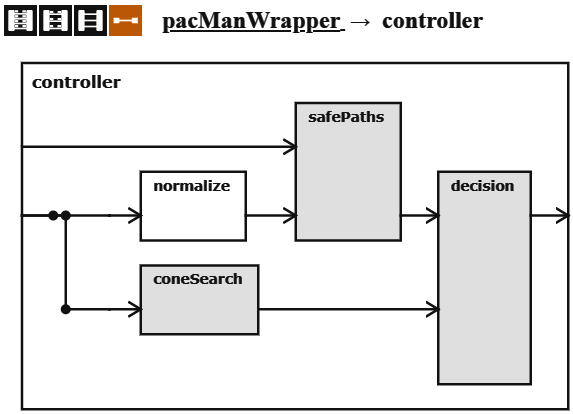
\includegraphics[scale=0.85]{pictures/Pacman/Controller20.png}
\end{figure}

The more complex Pacman controller is shown in fig. \ref{fig:visPacman20}.
It has three main subcomponents:
\begin{itemize}
	\item \textit{safePaths}: This component is responsible for checking all the paths leading from Pacman into the labyrinth for safety. This is done by searching in each of the four possible directions until a wall or intersection is found.	
	\item \textit{coneSearch}: Searches in cones in each of the four directions for enemies and coins and gives back a score for each direction.	
	\item \textit{decision}: The decision component evaluates all data from the other two components. Based on those values it decides which direction the Pacman should go next.	
\end{itemize}
The last component \textit{normalize} not listed here is only responsible for increasing all position values from the ghosts and Pacman by 1 to fit the indexation from the math library.
We will now go into detail for the three main component.
\newline

\emph{Safe Paths} \newline
\begin{figure}
	\caption{Visualization of Safe Paths}
	\label{fig:safePaths}
	\centering
	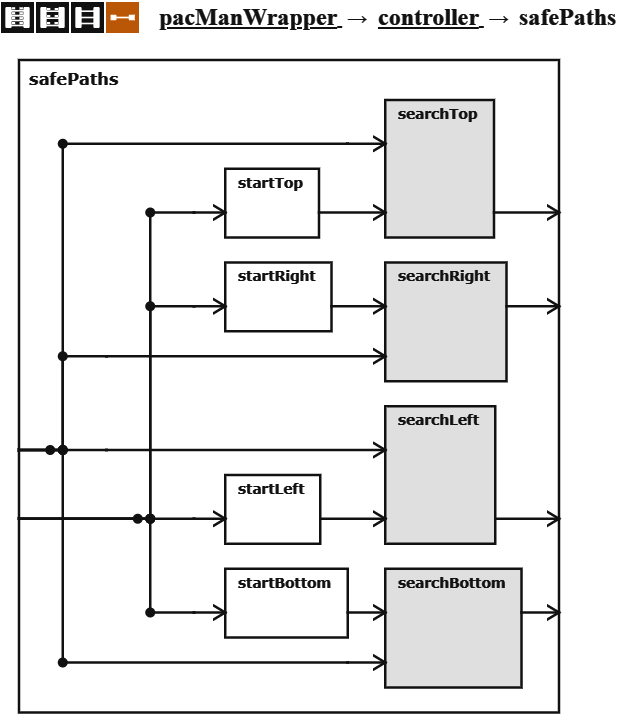
\includegraphics[scale=0.75]{pictures/Pacman/safePaths.png}
\end{figure}
In fig. \ref{fig:safePaths} the \textit{safePaths} component is shown. It contains a subcomponent for each direction and some starting values. It gives back whether the four directions are safe or not. A direction is safe if there is a wall blocking it (no path) or there is no enemy on its path until the next intersection. This is calculated by ``going'' the path. This could be done with a single component looping through the path to the next intersection. Due to the fact that this would contradict the conditions on C\&C components stated before it is split up into subcomponents. Each path in this labyrinth has a length of at most 10. So the task is divided into 10 components as one can partially see in fig. \ref{fig:search}. Each of those checks whether the current position is safe and then calculate the position to check for the next component. This way the runtime is fixed and the code is better parallelizable.
\begin{figure}
	\caption{Visualization of one Search}
	\label{fig:search}
	\centering
	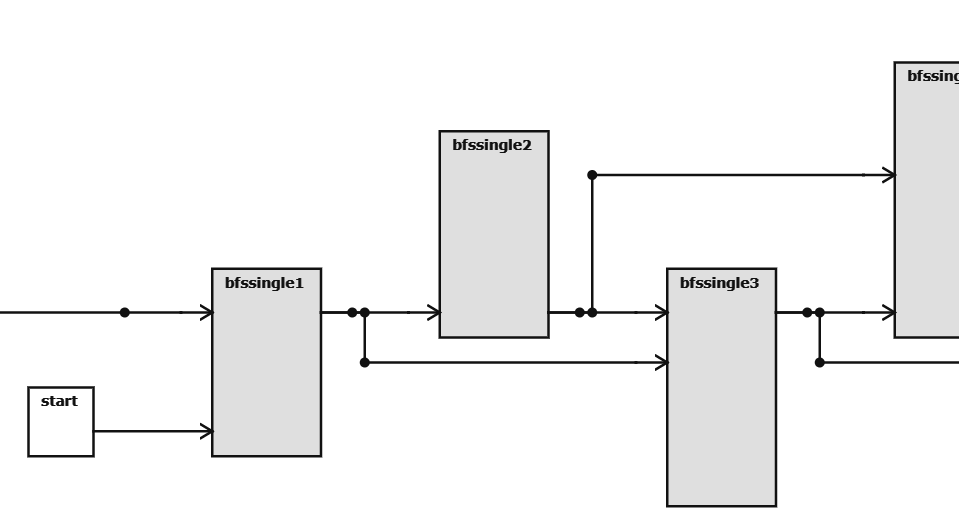
\includegraphics[scale=0.5]{pictures/Pacman/Search.png}
\end{figure}

\begin{figure}
	\caption{Visualization of one Single Search Component}
	\label{fig:searchSingle}
	\centering
	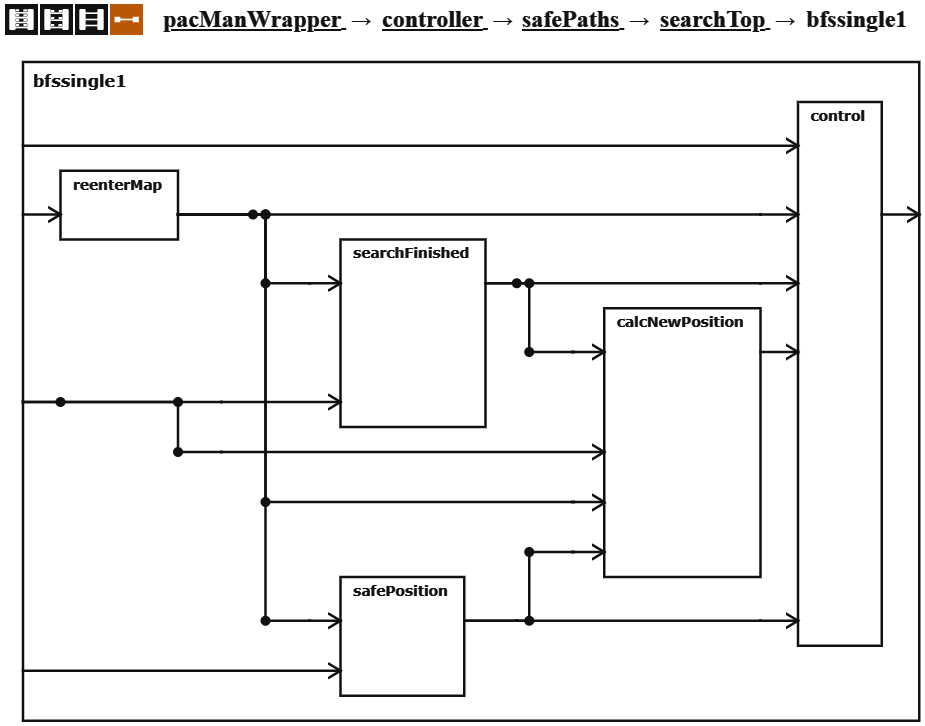
\includegraphics[scale=0.55]{pictures/Pacman/SearchSingle.png}
\end{figure}
The task of one of the 10 subcomponents is again split up into 5 subtasks (see fig. \ref{fig:searchSingle}):
\begin{itemize}
	\item \textit{reenterMap}: If the previous component calculated a position outside of the map (e.g. leaving the map on the right through the tunnel), reenter the map on the other side.
	\item \textit{safeFinished}: The search is finished if it is marked as finished by a previous search component or a wall is found (only when there is no path).
	\item \textit{safePosition}: Loops through the four ghosts and check whether their position matches the current position. If an unsafe tile is found, the search is marked as finished and not safe.
	\item \textit{calcNewPosition}: Looks for free ways in the adjacent tiles. If there are more than two free tiles (no wall), an intersection is reached and the search can be marked finished. Otherwise this component gives back the next position which is different from the previous one.
	\item \textit{control}: The control unit evaluates all data from the other components and gives back a corresponding new position and whether the search until now is safe or not.
\end{itemize}

\emph{Cone Search} \newline
\begin{figure}
	\caption{Visualization of Cone Search}
	\label{fig:cone}
	\centering
	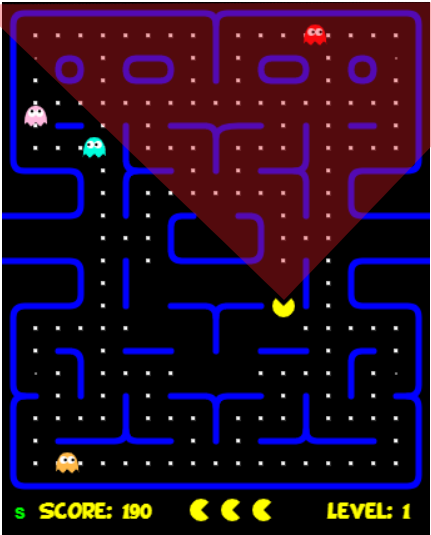
\includegraphics[scale=0.65]{pictures/Pacman/Cone.png}
\end{figure}
The \textit{ConeSearch} component searches through the map in cones (see fig. \ref{fig:cone}). This way each direction can be given a value which increases when biscuits and coins are found and decreases when ghosts are found. The following weights are used in the most current version:
\begin{itemize}
	\item biscuit: 50
	\item coin: 200
	\item enemy (facing towards Pacman): -10
	\item enemy (facing a different direction): -4
	\item enemy (eatable): 1000
\end{itemize}
The values shrink with the distance to Pacman. The biscuit/coin value shrink squared and the enemy value linear with the distance. This way near objectives are valued more and Pacman does not go for only far away biscuits/coins if there already are nearby ones. But if all biscuit/coin values are small the maximum gets increased by a fix amount, so Pacman goes for far away biscuits/coins if there are no around. In the end for each direction a value is returned by combining the biscuits/coins value and the enemy value. 
\begin{figure}
	\caption{Visualization of Cone Search}
	\label{fig:coneSearch}
	\centering
	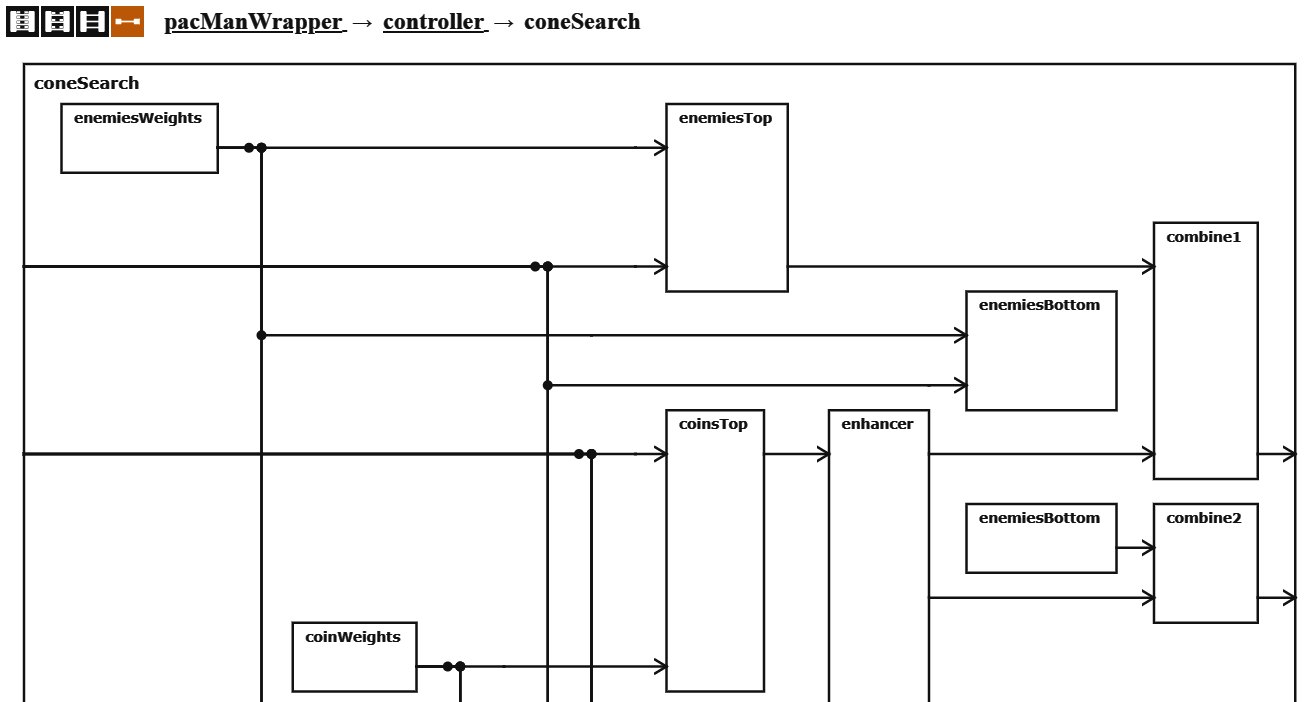
\includegraphics[scale=0.55]{pictures/Pacman/ConeSearch.png}
\end{figure}

In the visualization of the component (see fig. \ref{fig:coneSearch}) one can see the different kind of subcomponents:
\begin{itemize}
	\item \textit{enemiesWeights} and \textit{coinWeights}: some constants for weighting biscuits, coins and ghost values. This design allows easy adjustments.
	\item \textit{enemies(Top)}: searches for enemies in the (top) cone and gives back its value.
	\item \textit{coins(Top)}: searches for biscuits/coins in the (top) cone and gives back its value.
	\item \textit{enhancer}: increases the maximum biscuits/coins value if it is small.
	\item \textit{combine}: combines the values for biscuits/coins and enemies for a direction.
\end{itemize}

\emph{Decision} \newline
\begin{figure}
	\caption{Visualization of Cone Search}
	\label{fig:decision}
	\centering
	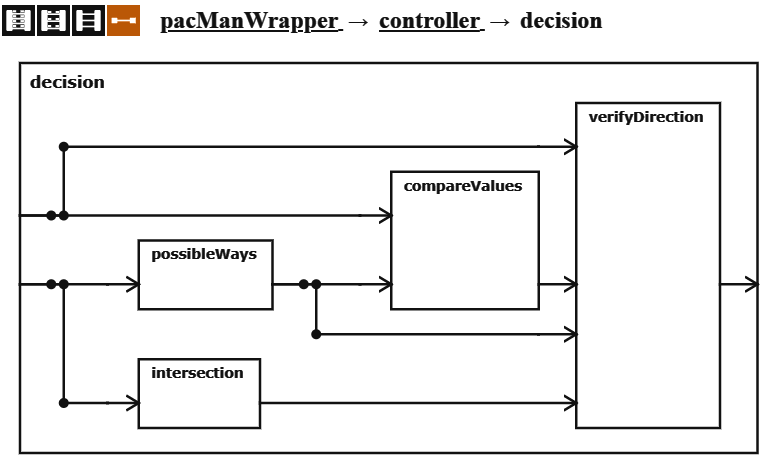
\includegraphics[scale=0.55]{pictures/Pacman/Decision.png}
\end{figure}
The \textit{decision} component gets all data from \textit{safePaths} and \textit{coneSearch} and makes a final decision on where to go. Beside the maximum value for a direction and whether it is safe or not, the decision is based on a few additional information. E.g. the top direction has the maximum value from the cone searches but it is blocked by a wall or not safe. Then another direction has to be chosen. Here an orthogonal direction (left or right) is preferred to stay near to the desired one (top). In addition, to prevent stuttering a new path is only chosen if the current one is not safe anymore or an intersection is reached.
In fig. \ref{fig:decision} one can see the four subcomponents of \textit{safePaths}:
\begin{itemize}
	\item \textit{intersection}: Gives back whether Pacman is located on a tile with more than 2 Paths leading from it.
	\item \textit{possibleWays}: Gives back which directions are not blocked by a wall.
	\item \textit{compareValues}: Calculates the safe direction with the maximum value. If this direction is blocked, a new direction has to be chosen.
	\item \textit{verifyDirection}: Checks whether the chosen direction is opposing the previous one. This is only allowed if the previous direction is not safe anymore or an intersection is reached.
\end{itemize}


\newpage
\subsection{ Modeling - Supermario (by Philipp Haller)}

This part discusses the model used to solve a level of the Supermario game which was presented in section XX. First a general introduction on model types is given. Thereafter, the different models are discussed step by step, beginning at the most abstract.

\subsubsection{Simulator Interface}


\subsubsection{Model Types}

In this context the following model types used were:
\newline

\emph{Watcher} \newline
The watcher model type takes a position as input and returns a boolean value which indicates if it is in a certain range.
\newline

\emph{Selector} \newline
The selector model type uses a raw array and an index as input and returns the corresponding array entry.
\newline

\emph{Strategy} \newline
A strategy model type can take different inputs and performs a action decision based on its inputs.
\newline

\emph{Controller} \newline
The controller model type combines the other defined model types to refine the inputs of the simulation and executes a strategy.
\newline

\emph{Filter} \newline
The filter model type is intended to perform filtering like debouncing and plausibility checks.

\subsubsection{Models}
The presented model visualizations are generated from the EmbeddedMontiArc Studio. Therein, a grey component indicates that the component uses additional subcomponents, whereas a white component marks atomic components. 

Split -> Reference

The first and most abstract entity modeled was the supermario wrapper which is closely related to the outputs and inputs of the simulator. Therefore it receives all necessary values as input with the aim to forward them to the actual controller and its corresponding sub-components. After computation the results of the controller are handed back into the wrapper, which forwards the data to the simulator. Figure \ref{fig:marioWrapper} shows the graphical representation, while listing \ref{lst:marioWrapperInterface} shows the actual EMA interface definition.
\begin{figure}
	\centering
	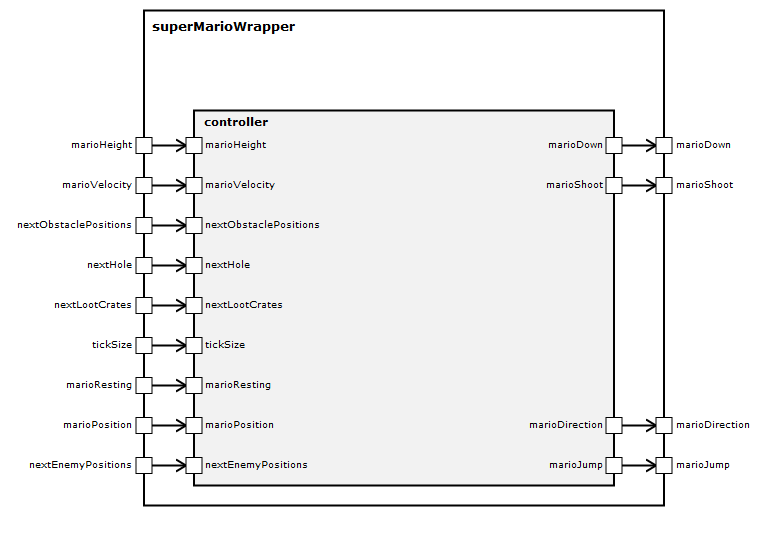
\includegraphics[scale=0.5]{pictures/haller_supermariowrapper.PNG}
	\caption{Visualisation of the Supermario wrapper model}
	\label{fig:marioWrapper}
\end{figure}

\begin{lstlisting}[label=lst:marioWrapperInterface, caption=Interface of the Supermario Wrapper, morekeywords={ports, port, connect, in, out, instance, ->},
frame=single]
    ports   
        in Z^{1,2} marioPosition,
        in Z^{1,2} marioVelocity,
        in Z marioHeight,
        in Z^{5,2} nextEnemyPositions,
        in Z^{5,2} nextObstaclePositions,
        in Z nextHole,
        in Z^{5,2} nextLootCrates,
        in Q tickSize,
        in Z marioResting,
        out Z(-1 : 1 : 1) marioDirection,
        out Z marioJump,
        out Z marioDown,
        out Z marioShoot;
\end{lstlisting}

The player figure's position, velocity and height were chosen as inputs, together with the positions of the next five enemies and obstacles. Furthermore, the position of the next hole in the ground, the position of the next five loot crates, the tick size (the time between model executions) and the information if the player is resting on a tile is given.
The outputs consist of the direction the player shall go in combination with the action instructions jumping, crouching and shooting.
The data type for most values is integer, indicated by a "Z" in the code. This is due to the circumstance that the simulator uses a number of pixels as a measure for distance. Only exception being the "tickSize" which can be fractions of a second.

\begin{figure}
	\centering
	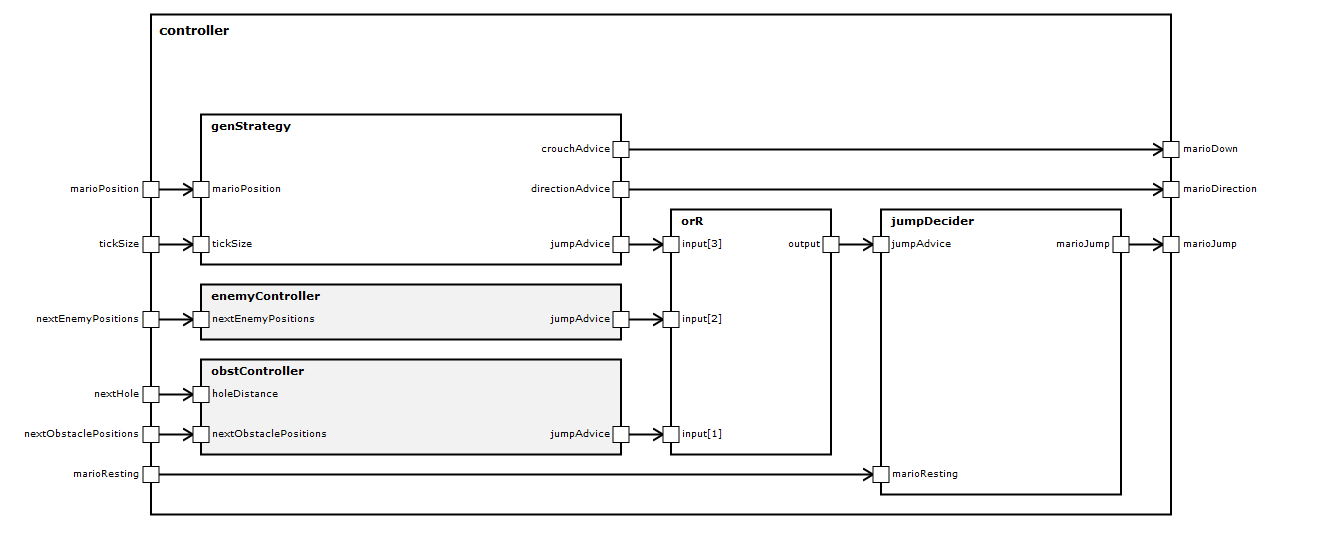
\includegraphics[scale=0.5]{pictures/haller_controller.PNG}
	\caption{Visualization of the Supermario controller model}
	\label{fig:marioController}
\end{figure}

The controller used (Figure \ref{fig:marioController}) consists of five parts and is depicted in figure XX. There are sub-controllers tasked to cope with the evaluation of enemies and obstacles respectively, named enemyController and obstController. They return an advice to indicate if the player should jump or not. The genStrategy is an atomic component which is currently used to provide a general strategy like moving in another direction, jumping or crouching if the player is stuck. 

The action advices of the controllers and the strategy are combined via a logical or-relation, as indicated by the "orR" block. Additionally, the jumpDecider filters the output of the combined value and forwards it, if the player can jump in that time frame. This is necessary to prohibit side-effects like the player only jumping once because the jump key remains pressed constantly and the simulator only accepts distinct jump activations, opposed to continuous jumping.

\begin{figure}
	\centering
	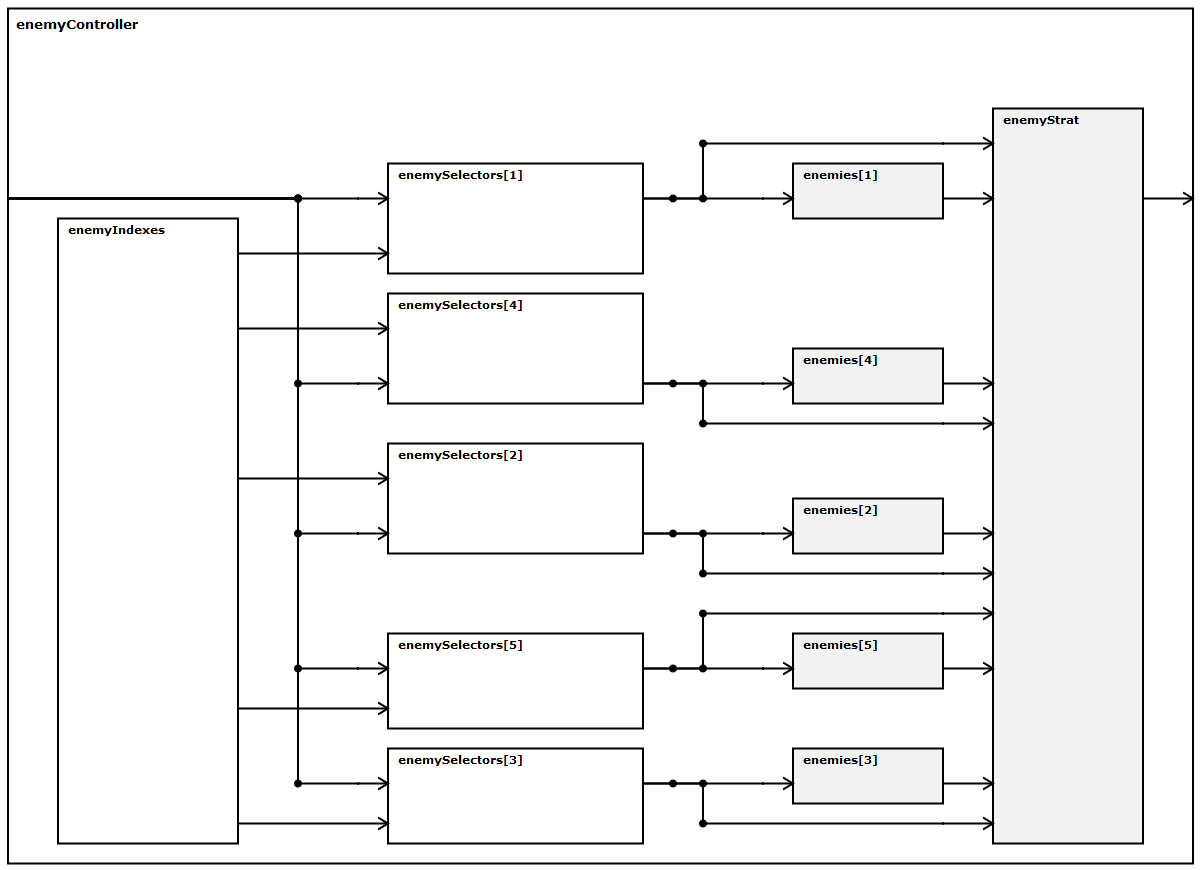
\includegraphics[scale=0.4]{pictures/haller_enemycontroller.PNG}
	\caption{Visualization of the Supermario enemy controller model}
	\label{fig:marioEnemyController}
\end{figure}

The enemy controller (Figure \ref{fig:marioEnemyController}) handles the enemy position evaluation and assesses if an action has to be initiated. As the input data from the simulator is a array with five positions, it contains a enemy selector component which returns the corresponding x and y values from a given index. For purposes of overview and readability of the EMA code a component "enemyIndexes" was used to feed these indexes into the selectors.

\begin{figure}
	\centering
	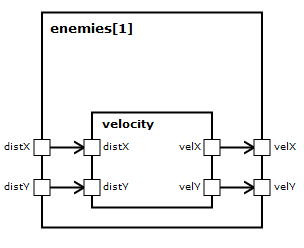
\includegraphics[scale=0.5]{pictures/haller_enemy.PNG}
	\caption{Visualization of the Supermario enemy model}
	\label{fig:marioEnemy}
\end{figure}

The enemy component (Figure \ref{fig:marioEnemy}) is used to compute a velocity from the x and y positions by comparing the former positions with the current ones.

\begin{figure}
	\centering
	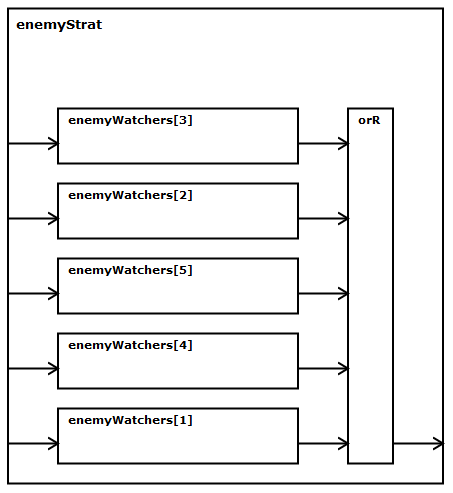
\includegraphics[scale=0.4]{pictures/haller_enemystrategy.PNG}
	\caption{Visualization of the Supermario enemy strategy model}
	\label{fig:marioEnemyStrategy}
\end{figure}

The enemy strategy (Figure \ref{fig:marioEnemyStrategy}) uses the distances and velocities from the enemy components to watch them for their distance to the player and wether they can get dangerous. If an enemy comes too close and is on the player's plane, a jump advice is given. The jump advices are again combined via a logical or-relation and returned.

\begin{figure}
	\centering
	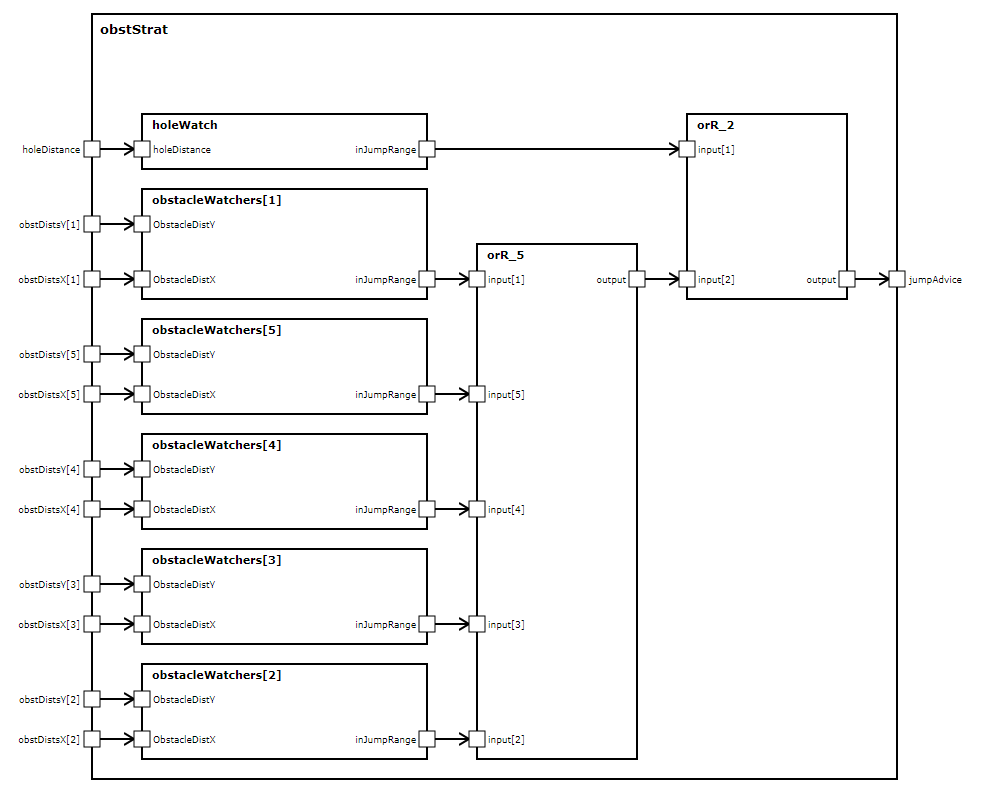
\includegraphics[scale=0.4]{pictures/haller_obstaclestrategy.PNG}
	\caption{Visualization of the Supermario enemy strategy model}
	\label{fig:marioObstacleStrategy}
\end{figure}

The obstacle controller is modeled very similar to the enemy controller, extracting positions from the raw input array and feeding them into a obstacle strategy. The main difference to the enemy controller is the presence of another input. This additional input is the distance to the next hole in the ground plane of the level. It is forwarded into the obstacle strategy (Figure \ref{fig:marioObstacleStrategy}) where a watcher component checks the player's proximity to the hole and computes a jump advice. All advices are again combined by a or relation.


\subsubsection{Future Modeling}

The models presented in this chapter were developed with modularity and extensibility in mind, such that in future work more complex strategies can be used to solve more levels and to lay more attention to the score.
-mario direction
-weighted combination of decisions


\section{Evaluation (by Malte Heithoff)}
\label{sec:evaluation}
The two developers of Pacman and Supermario were interviewed in the manner mentioned in the introduction. In this section the results of this interviews are collected and summarized.

\subsection{RQ1 - Is EmbeddedMontiArc suitable for other systems?}
The tasks were both based on real-time problems which the EMA language is designed for. Both developers were able to model a controller which can beat a level in their specific domain. The code for the models is clearly and good readable. The generated Javascript code is fast enough to be executed every tick of the simulation (30 fps/ 60 fps). Based on the examples of Pacman and Supermario it is clear that real-time problems can be solved with EmbeddedMontiArc.

\subsection{RQ2 - Is it possible to integrate other simulators in a recent amount of work?}
To integrate the Pacman- and Supermario simulators two tasks had to be completed: integrate into the IDE and then link the simulator to the web assembly. The integration into the IDE was quite simple for both systems as soon as the instructions were handed out. But as there was no infrastructure for generating the web assembly before this led to some extra effort by installing emscripten and writing the needed scripts. The Simulator for Pacman was easily adjustable so that the extraction of the needed information (e.g. Pacman position) was done in short time. In contrast, the underlying structure of the Supermario project in use was way more complex and needed a lot more effort to understand it. Linking the web assembly with the simulator was done within little work as soon as the interface for extracting the data from the simulators and inputting the computed results was implemented. Just the data had to be transformed into the correct format and then the web assembly needed to be executed.

Therefore the answer to this question is dependent on the complexity of the system and on whether the is a working interface for extracting data. Pacman was fairly easy to integrate but Supermario needed more time than calculated.

\subsection{RQ3 - What kind of background knowloedge is needed to model C\&C in EMA?}
One of the developers had some experience with EmbeddedMontiArc while the other had not. Both are computer science students and are therefore familiar with programming concepts and the modular programming that EMA requires. For the more experienced developer the concept of C\&C was easy to understand and he could easily make use some of the tooling the language offers. The less experienced developer had a few problems in the beginning but after overcoming those he had no further problems with implementing what he was trying to. Both developers benefited from being familiar with programming languages so the math library was easy to understand. 

Having experience with programming concepts is necessary to model C\&C in EMA but specific knowledge about the EMA language is optional and can be obtained in a short time.

\subsection{RQ4 - What features are good and what are not suited?}
This section will be split up into the question about the tools around the language and the question about the features the language itself is offering.

\subsubsection{Tools}
The onlineIDE coming with the EmbeddedMontiArcStudio is powerful enough to help with the modeling process. But it is also missing a lot of tools a modern ide is offering. The safe option was also one of the weak points of the ide, only after running a plugin all the files are saved to the hard drive. Syntax checking was sufficient for the non-atomic components but missing for the atomic components. The other tools integrated into the ide, such as generating a report with semantical checks of the models or generating a visualization could be utilized for error checking and planning the model. But most of the tools had a long runtime and need optimization.

\subsubsection{Language Features}
The option to import other components and to have a package hierarchy were used all the time and are well suited for the purpose of the language. Also connecting arrays of ports with a [:] is very convenient but this option is not nested which made the code at some point larger than necessary. What was missing in this version of the code generator is the ability to use structs as a port type which led to unclear port interface for some components.

All in all, the features the ide and the language were offering helped with the modeling process and are well suited for the language purpose.

\subsection{Other Problems}
Although in theory there are no major problems with modeling the two groups had to fight some bugs in the code generation process. Most of those bugs are fixed by now, but at the time of modeling led to some considerable time losses. Due to the fact that the transformation from the C++ code to Javascript had a really long runtime, testing the code needed a lot of time as well.





\section{Conclusion (by Haller and Heithoff)}
\label{sec:conclusion}
This section is going to be written in the near future

\newpage
\appendix
\section{Pacman EmbeddedMontiArc Code}
\begin{figure}[H]
	\centering
	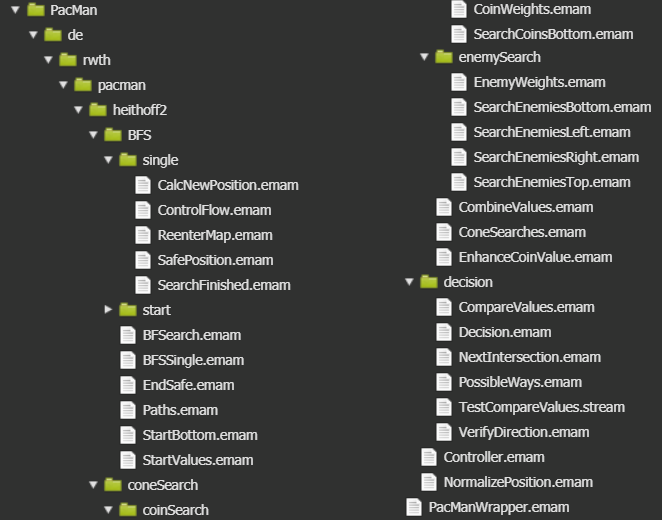
\includegraphics[scale=1]{pictures/Pacman/heithoff_pacmanoutlineSmall.PNG}
	\caption{Pacman package outline}
	\label{fig:pacmanpackageoutline}
\end{figure}

\lstinputlisting[caption=PacmanWrapper]{model/pacman/PacManWrapper.emam}
\lstinputlisting[caption=Controller]{model/pacman/heithoff2/Controller.emam}
\lstinputlisting[caption=NormalizePosition]{model/pacman/heithoff2/NormalizePosition.emam}
\lstinputlisting[caption=BFS.BFSearch]{model/pacman/heithoff2/BFS/BFSearch.emam}
\lstinputlisting[caption=BFS.BFSSingle, basicstyle=\footnotesize]{model/pacman/heithoff2/BFS/BFSSingle.emam}
\lstinputlisting[caption=BFS.EndSafe]{model/pacman/heithoff2/BFS/EndSafe.emam}
\lstinputlisting[caption=BFS.Paths, basicstyle=\footnotesize]{model/pacman/heithoff2/BFS/Paths.emam}
\lstinputlisting[caption=BFS.StartBottom]{model/pacman/heithoff2/BFS/StartBottom.emam}
\lstinputlisting[caption=BFS.StartValues]{model/pacman/heithoff2/BFS/StartValues.emam}
\lstinputlisting[caption=BFS.single.CalcNewPosition]{model/pacman/heithoff2/BFS/single/CalcNewPosition.emam}
\lstinputlisting[caption=BFS.single.ControlFlow]{model/pacman/heithoff2/BFS/single/ControlFlow.emam}
\lstinputlisting[caption=BFS.single.ReenterMap]{model/pacman/heithoff2/BFS/single/ReenterMap.emam}
\lstinputlisting[caption=BFS.single.SafePosition]{model/pacman/heithoff2/BFS/single/SafePosition.emam}
\lstinputlisting[caption=BFS.single.SearchFinished]{model/pacman/heithoff2/BFS/single/SearchFinished.emam}
\lstinputlisting[caption=coneSearch.CombineValues]{model/pacman/heithoff2/coneSearch/CombineValues.emam}
\lstinputlisting[caption=coneSearch.ConeSearches]{model/pacman/heithoff2/coneSearch/ConeSearches.emam}
\lstinputlisting[caption=coneSearch.EnhanceCoinValue]{model/pacman/heithoff2/coneSearch/EnhanceCoinValue.emam}
\lstinputlisting[caption=coneSearch.coinSearch.CoinWeights]{model/pacman/heithoff2/coneSearch/coinSearch/CoinWeights.emam}
\lstinputlisting[caption=coneSearch.coinSearch.SearchCoinsBottom]{model/pacman/heithoff2/coneSearch/coinSearch/SearchCoinsBottom.emam}
\lstinputlisting[caption=coneSearch.enemySearch.EnemyWeights]{model/pacman/heithoff2/coneSearch/enemySearch/EnemyWeights.emam}
\lstinputlisting[caption=coneSearch.enemySearch.SearchEnemiesBottom]{model/pacman/heithoff2/coneSearch/enemySearch/SearchEnemiesBottom.emam}

\lstinputlisting[caption=decision.CompareValues, basicstyle=\scriptsize ]{model/pacman/heithoff2/decision/CompareValues.emam}
\lstinputlisting[caption=decision.Decision]{model/pacman/heithoff2/decision/Decision.emam}
\lstinputlisting[caption=decision.NextIntersection]{model/pacman/heithoff2/decision/NextIntersection.emam}
\lstinputlisting[caption=decision.PossibleWays]{model/pacman/heithoff2/decision/PossibleWays.emam}
\lstinputlisting[caption=decision.VerifyDirection]{model/pacman/heithoff2/decision/VerifyDirection.emam}

\subsection{Pacman Stream Test Code}
\lstinputlisting[caption=decision.TestCompareValues]{model/pacman/heithoff2/decision/TestCompareValues.stream}
\lstinputlisting[caption=Flee down]{PMStream/Scenarien/01/Test1.stream}
\lstinputlisting[caption=Flee left]{PMStream/Scenarien/02/Test2.stream}
\lstinputlisting[caption=Eat ghosts]{PMStream/Scenarien/03/Test3.stream}
\lstinputlisting[caption=Eat biscuits]{PMStream/Scenarien/04/Test4.stream}
\lstinputlisting[caption=Eat coin]{PMStream/Scenarien/05/Test5.stream}

\newpage
\section{Supermario EmbeddedMontiArc Code}
\begin{figure}[!h]
	\centering
	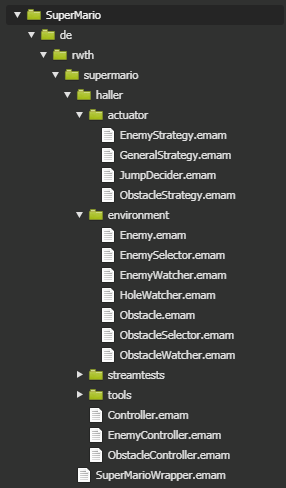
\includegraphics[scale=1]{pictures/haller_mariooutline.PNG}
	\caption{Supermario package outline}
	\label{fig:mariopackageoutline}
\end{figure}
\pagebreak
\lstinputlisting[caption=SuperMarioWrapper]{model/supermario/SuperMarioWrapper.emam}
\pagebreak
\lstinputlisting[caption=Controller]{model/supermario/haller/Controller.emam}
\pagebreak
\lstinputlisting[caption=EnemyController]{model/supermario/haller/EnemyController.emam}
\pagebreak
\lstinputlisting[caption=ObstacleController]{model/supermario/haller/ObstacleController.emam}
\pagebreak
\lstinputlisting[caption=actuator.GeneralStrategy]{model/supermario/haller/actuator/GeneralStrategy.emam}
\pagebreak
\lstinputlisting[caption=actuator.EnemyStrategy]{model/supermario/haller/actuator/EnemyStrategy.emam}
\pagebreak
\lstinputlisting[caption=actuator.ObstacleStrategy]{model/supermario/haller/actuator/ObstacleStrategy.emam}
\pagebreak
\lstinputlisting[caption=actuator.JumpFilter]{model/supermario/haller/actuator/JumpFilter.emam}
\pagebreak
\lstinputlisting[caption=environment.Enemy]{model/supermario/haller/environment/Enemy.emam}
\pagebreak
\lstinputlisting[caption=environment.EnemySelector]{model/supermario/haller/environment/EnemySelector.emam}
\pagebreak
\lstinputlisting[caption=environment.EnemyWatcher]{model/supermario/haller/environment/EnemyWatcher.emam}
\pagebreak
\lstinputlisting[caption=environment.HoleWatcher]{model/supermario/haller/environment/HoleWatcher.emam}
\pagebreak
\lstinputlisting[caption=environment.Obstacle]{model/supermario/haller/environment/Obstacle.emam}
\pagebreak
\lstinputlisting[caption=environment.ObstacleSelector]{model/supermario/haller/environment/ObstacleSelector.emam}
\pagebreak
\lstinputlisting[caption=environment.ObstacleWatcher]{model/supermario/haller/environment/ObstacleWatcher.emam}
\pagebreak
\lstinputlisting[caption=tools.GetVelocity]{model/supermario/haller/tools/GetVelocity.emam}
\pagebreak
\lstinputlisting[caption=tools.GetNearest]{model/supermario/haller/tools/GetNearest.emam}


\subsection{Supermario Stream Test Code}
\begin{lstlisting}[label=lst:enemywatchertest_1, caption=Enemy watcher stream test, morekeywords={package, stream, tick, for},
frame=single, basicstyle=\small]
package de.rwth.supermario.haller.environment;

stream Env_EnemyWatcher_Evade for EnemyWatcher {
    EnemyDistX:         200 tick    100     tick     75;
    EnemyDistY:           0 tick      0     tick      0;
    EnemyVelocityX:     -10 tick    -10     tick    -10;
    EnemyVelocityY:       0 tick      0     tick      0;
            
    movesTowardsPlayer:   1 tick      1     tick      1;
    inJumpRange:          0 tick      0     tick      1;
    }
\end{lstlisting}

\begin{lstlisting}[label=lst:enemywatchertest_2, caption=Enemy watcher stream test, morekeywords={package, stream, tick, for},
frame=single, basicstyle=\small]
package de.rwth.supermario.haller.environment;

stream Env_EnemyWatcher_FromAbove for EnemyWatcher {
        
    EnemyDistX:         200 tick    100     tick      5;
    EnemyDistY:         128 tick    128     tick     32;
    EnemyVelocityX:     -10 tick    -10     tick    -10;
    EnemyVelocityY:       0 tick      0     tick      0;
            
    movesTowardsPlayer:   1 tick      1     tick      1;
    inJumpRange:          0 tick      0     tick      0;

    }
\end{lstlisting}

\begin{lstlisting}[label=lst:enemywatchertest_3, caption=Enemy watcher stream test, morekeywords={package, stream, tick, for},
frame=single, basicstyle=\small]
package de.rwth.supermario.haller.environment;

stream Env_EnemyWatcher_FromAbove for EnemyWatcher {
        
    EnemyDistX:         -1 tick;
    EnemyDistY:         -1 tick;
    EnemyVelocityX:      0 tick;
    EnemyVelocityY:      0 tick;
            
    movesTowardsPlayer:  0 tick;
    inJumpRange:         0 tick;

    }
\end{lstlisting}

\begin{lstlisting}[label=lst:obstaclewatchertest, caption=Obstacle watcher stream test, morekeywords={package, stream, tick, for},
frame=single, basicstyle=\small]
package de.rwth.supermario.haller.environment;
stream Env_ObstacleWatcher for ObstacleWatcher {
  ObstacleDistX: 200 tick 100 tick 75 tick 50 tick 25 tick  0;
  ObstacleDistX:   0 tick   0 tick  0 tick 25 tick 50 tick 75;
    
  inJumpRange:     0 tick   0 tick  1 tick  1 tick  1 tick  0;
    }
\end{lstlisting}

\begin{lstlisting}[label=lst:holewatchertest, caption=Hole watcher stream test, morekeywords={package, stream, tick, for},
frame=single, basicstyle=\small]
package de.rwth.supermario.haller.environment;
stream Env_ObstacleWatcher for ObstacleWatcher {
    holeDistance: 200 tick 100 tick 10 tick 0 tick 1200;
    
    inJumpRange:    0 tick   0 tick  1 tick	1 tick    0;
    }
\end{lstlisting}

\newpage
\section*{References}
\bibliography{bibliography}



\end{document}